\documentclass[11pt, a4paper]{article}
\usepackage[utf8]{inputenc}
\usepackage[margin=1in]{geometry}
\usepackage[toc, page]{appendix}
\usepackage{multirow}
\usepackage{pdflscape}
\usepackage{array}
\usepackage{longtable}
\usepackage{color} 
\usepackage[pdftex]{hyperref}
\hypersetup{
	colorlinks=true,
	linktoc=all,
	linkcolor=black,
	citecolor=black,
}
\usepackage[export]{adjustbox}
\usepackage{float}
\restylefloat{table}
\usepackage{array}
\usepackage[final]{microtype}
\usepackage{tikz}
\usepackage{graphicx}
\usepackage{pgfplots}
\pgfplotsset{compat=newest}
\usepackage{filecontents}
\usepackage{multirow}
\usepackage{callouts}
\usepackage{longtable}
\usepackage{array}
\usepackage[justification=centering]{caption} 
\usetikzlibrary{intersections}
\usepackage{fontawesome}
\usepackage{capt-of}
\usepackage{setspace}
\usepackage{tablefootnote}
\usepackage{subcaption}
\usepackage[style=mla, backend=biber]{biblatex}
\usepackage{caption}
\captionsetup[figure]{font=footnotesize}
\captionsetup[table]{font=footnotesize}
\usepackage{wrapfig}
\usepackage{scrextend}
\usepackage[normalem]{ulem}
\useunder{\uline}{\ul}{}
\deffootnote{0em}{1.6em}{\thefootnotemark.\enskip}

\title{MYP Economics G2 01 - Microeconomics Commentary}
\author{Adithya Narayanan}
\date{4 May, 2020}

\begin{document}
	\begin{titlepage}
		\maketitle

		\begin{center}
			\large How the electronics supply chain is responding to COVID-19 in China

			Word count: 749
		\end{center}
		\thispagestyle{empty}
	\end{titlepage}
	
	\newpage
	\tableofcontents
	\thispagestyle{empty}
	\newpage
	\clearpage
	\setcounter{page}{1}
	\setcounter{secnumdepth}{0}
	\section{Article:}
		\textbf{\footnotesize SUPPLY CHAIN}
		
		\bigbreak
		\noindent
		\textbf{\LARGE How the Electronics Supply Chain is Responding to COVID-19}
		\noindent
		\newline
		\textit{What companies worldwide are doing to help shore up the electronics supply chain during these times of extreme uncertainty.}
		
		\bigbreak
		\noindent
		Bridget McCrea
		\newline
		\noindent
		APR 08, 2020

		\bigbreak
		
		As the COVID-19 pandemic continues to take its toll on human lives, livelihoods and economies worldwide, the electronics industry is making moves to shore up supply chains and ensure a smooth transition when commerce returns to a more normalized state. The component shortage that took hold long before the pandemic emerged is making that task more difficult for manufacturers and distributors alike.
		\bigbreak
		“Shortages of components and raw materials because of the coronavirus are likely to be far worse than expected, with most US companies unaware that they are exposed to Chinese factories idled by the outbreak,” Financial Times points out. “I guarantee you that most organizations have some level of exposure that they are not aware of,” Ivalua’s Alex Saric told the publication.
		
		\subsection{Close Tracking}

			Financial Times goes on to explain that while companies closely track their direct suppliers—the tier ones such as Foxconn that sends Apple a finished iPhone—“they can be blind to their suppliers’ factories, the tier twos, and those further down the chain.”
			\bigbreak
			In fact, it says one Bain \& Co. analyst estimates that 60\% of executives lack any supply chain visibility beyond their tier one suppliers. This can become a major issue in a world where Resilinc says about 1,800 manufactured parts originate in the quarantined areas of China that are centered around Hubei province. 
			\bigbreak
			“The scariest thing we see is the highest numbers of parts [made in and around Hubei] are caps and resistors — tiny things nobody cares about — plus thermal components, plastics and resins, and sheet metals,” Resilinc’s Bindiya Vakil told Financial Times, which advises companies to prepare now for six months of supply chain disruptions.   

		\subsection{Back to China}

			With its role in the national pandemic now waning, China is becoming a focal point for electronics makers that are scrambling to shore up their supply chains. According to Forbes,
			\bigbreak
			iPhone maker Foxconn says its China plants can meet seasonal demand after finding enough workers since the country shed the worst of its coronavirus outbreak in February and early March.
			\bigbreak
			“Demand could surface in China, too, as companies there start placing orders again for domestic consumers who can go outside now after a dismal February,” Forbes reports. “Foxconn will still keep China as [its] manufacturing base and focus on the domestic market for their consumer-facing business, whether it be brand or channel,” Quantum International’s John Brebeck told Forbes.
			\bigbreak
			The Verge says Foxconn was at reduced capacity for most of February and is hoping to get back to full strength by the end of the month. “But with so many other manufacturers still scaling up, the result is a huge disruption in the supply chain,” it points out in “Electronics companies are getting gridlocked by coronavirus lockdowns.”
			\bigbreak
			The situation is being made worse by the structure of modern manufacturing, The Verge adds. “For decades, hardware companies have been cutting costs by reducing stockpiles, trying to minimize the time a product spends sitting around at any stage of the process,” it reports. “That magnifies the impact of any disruption to the system, whether the component can’t be built because the workers are locked down or can’t be shipped as fast because of travel restrictions.”

			“The emergency airlift plans underscore the interconnected nature of global supply chains and the continued dependence on China for key goods,” it continues, “even as some manufacturers — prompted in some cases by the U.S.-China trade war — move to build up capacity outside of China.”

		\newpage

	\section{Commentary:}
		\begin{center}
			\textbf{\Large How the Electronics Supply Chain is Responding to COVID-19 in China}
		\end{center}
		
		The world's largest industry, in terms of market capitalization, witnessed supply chain shortages, as a result of an impaired global economy. The inability to meet demand, is a prime example of shortage.

		\subsection{Creation of a shortage:}
			A shortage occurs when the quantity demanded of a good is greater than quantity supplied, creating a state of market disequilibrium. The onset of a global pandemic resulted in a supply shock, with Factors of Production(FoPs) becoming nearly impossible to reallocate, especially labour, due to government intervention, resulting in overall lower quantities supplied to the market(See Fig.1).

			\begin{figure}[H]
				

\tikzset{every picture/.style={line width=0.75pt}} %set default line width to 0.75pt        

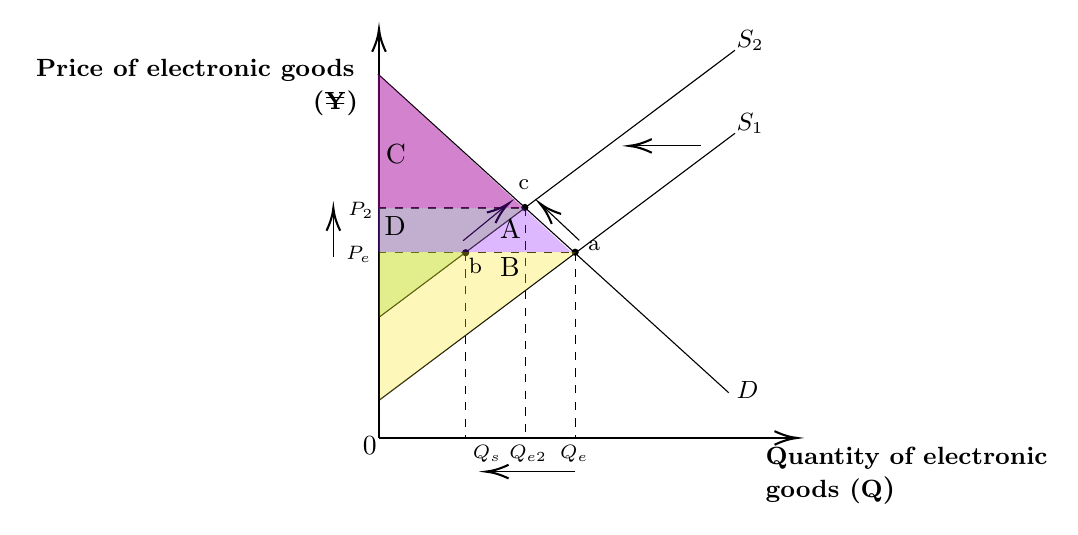
\begin{tikzpicture}[x=0.75pt,y=0.75pt,yscale=-1,xscale=1]
%uncomment if require: \path (0,255); %set diagram left start at 0, and has height of 255

%Straight Lines [id:da596173885597008] 
\draw    (228.5,30.38) -- (397.5,183.93) ;
%Straight Lines [id:da7602849312413997] 
\draw    (229,205.72) -- (229,10.72) ;
\draw [shift={(229,8.72)}, rotate = 450] [color={rgb, 255:red, 0; green, 0; blue, 0 }  ][line width=0.75]    (10.93,-3.29) .. controls (6.95,-1.4) and (3.31,-0.3) .. (0,0) .. controls (3.31,0.3) and (6.95,1.4) .. (10.93,3.29)   ;
%Straight Lines [id:da729313932578143] 
\draw    (229,205.72) -- (428.5,205.72) ;
\draw [shift={(430.5,205.72)}, rotate = 180] [color={rgb, 255:red, 0; green, 0; blue, 0 }  ][line width=0.75]    (10.93,-3.29) .. controls (6.95,-1.4) and (3.31,-0.3) .. (0,0) .. controls (3.31,0.3) and (6.95,1.4) .. (10.93,3.29)   ;
%Straight Lines [id:da9091680414856489] 
\draw    (384,65) -- (351.5,65) ;
\draw [shift={(349.5,65)}, rotate = 360] [color={rgb, 255:red, 0; green, 0; blue, 0 }  ][line width=0.75]    (10.93,-3.29) .. controls (6.95,-1.4) and (3.31,-0.3) .. (0,0) .. controls (3.31,0.3) and (6.95,1.4) .. (10.93,3.29)   ;
%Straight Lines [id:da13551280891737805] 
\draw  [dashed]  (228.5,116.48) -- (323.5,116.48) ;
%Straight Lines [id:da037485832122450935] 
\draw  [dashed]  (228.5,94.93) -- (299.5,94.93) ;
%Straight Lines [id:da34806942549457953] 
\draw  [dashed]  (299.5,94.93) -- (299.5,204.93) ;
%Straight Lines [id:da4293572932539924] 
\draw    (400.5,58.93) -- (229.13,187.48) ;
%Straight Lines [id:da2346975945434593] 
\draw    (400.5,18.93) -- (229.13,147.48) ;
%Straight Lines [id:da8153930295208949] 
\draw  [dashed]  (323.5,116.22) -- (323.5,205.72) ;
%Shape: Right Triangle [id:dp9617540704547674] 
\draw  [draw opacity=0][fill={rgb, 255:red, 208; green, 2; blue, 27 }  ,fill opacity=0.3 ] (228.5,30.38) -- (298.5,94.93) -- (228.5,94.93) -- cycle ;
%Straight Lines [id:da45367953457942045] 
\draw  [dashed]  (270.5,116.48) -- (270.5,205.72) ;
%Shape: Right Triangle [id:dp716913055315467] 
\draw  [draw opacity=0][fill={rgb, 255:red, 126; green, 211; blue, 33 }  ,fill opacity=0.3 ] (229.13,147.48) -- (299.5,94.93) -- (229.13,94.93) -- cycle ;
%Straight Lines [id:da5326069134955671] 
\draw    (323.5,221.93) -- (282.5,221.93) ;
\draw [shift={(280.5,221.93)}, rotate = 360] [color={rgb, 255:red, 0; green, 0; blue, 0 }  ][line width=0.75]    (10.93,-3.29) .. controls (6.95,-1.4) and (3.31,-0.3) .. (0,0) .. controls (3.31,0.3) and (6.95,1.4) .. (10.93,3.29)   ;
%Straight Lines [id:da8797860892796805] 
\draw    (269.5,110.71) -- (289.95,93.97) ;
\draw [shift={(291.5,92.71)}, rotate = 500.71] [color={rgb, 255:red, 0; green, 0; blue, 0 }  ][line width=0.75]    (10.93,-3.29) .. controls (6.95,-1.4) and (3.31,-0.3) .. (0,0) .. controls (3.31,0.3) and (6.95,1.4) .. (10.93,3.29)   ;
%Straight Lines [id:da742511241276935] 
\draw    (325.5,110.51) -- (307.96,94.08) ;
\draw [shift={(306.5,92.71)}, rotate = 403.14] [color={rgb, 255:red, 0; green, 0; blue, 0 }  ][line width=0.75]    (10.93,-3.29) .. controls (6.95,-1.4) and (3.31,-0.3) .. (0,0) .. controls (3.31,0.3) and (6.95,1.4) .. (10.93,3.29)   ;
%Shape: Circle [id:dp8476110814057312] 
\draw  [draw opacity=0][fill={rgb, 255:red, 0; green, 0; blue, 0 }  ,fill opacity=1 ] (321.76,116.22) .. controls (321.76,115.26) and (322.54,114.48) .. (323.5,114.48) .. controls (324.46,114.48) and (325.24,115.26) .. (325.24,116.22) .. controls (325.24,117.19) and (324.46,117.97) .. (323.5,117.97) .. controls (322.54,117.97) and (321.76,117.19) .. (321.76,116.22) -- cycle ;
%Shape: Circle [id:dp4955122432684427] 
\draw  [draw opacity=0][fill={rgb, 255:red, 0; green, 0; blue, 0 }  ,fill opacity=1 ] (269.01,116.48) .. controls (269.01,115.51) and (269.79,114.73) .. (270.76,114.73) .. controls (271.72,114.73) and (272.5,115.51) .. (272.5,116.48) .. controls (272.5,117.44) and (271.72,118.22) .. (270.76,118.22) .. controls (269.79,118.22) and (269.01,117.44) .. (269.01,116.48) -- cycle ;
%Shape: Circle [id:dp5272437431753039] 
\draw  [draw opacity=0][fill={rgb, 255:red, 0; green, 0; blue, 0 }  ,fill opacity=1 ] (299.5,95.18) .. controls (299.5,94.9) and (299.72,94.68) .. (300,94.68) .. controls (300.28,94.68) and (300.5,94.9) .. (300.5,95.18) .. controls (300.5,95.45) and (300.28,95.68) .. (300,95.68) .. controls (299.72,95.68) and (299.5,95.45) .. (299.5,95.18) -- cycle ;
%Shape: Circle [id:dp7266536912535058] 
\draw  [draw opacity=0][fill={rgb, 255:red, 0; green, 0; blue, 0 }  ,fill opacity=1 ] (297.51,94.68) .. controls (297.51,93.71) and (298.29,92.93) .. (299.26,92.93) .. controls (300.22,92.93) and (301,93.71) .. (301,94.68) .. controls (301,95.64) and (300.22,96.42) .. (299.26,96.42) .. controls (298.29,96.42) and (297.51,95.64) .. (297.51,94.68) -- cycle ;
%Shape: Right Triangle [id:dp5182436369352543] 
\draw  [draw opacity=0][fill={rgb, 255:red, 144; green, 19; blue, 254 }  ,fill opacity=0.3 ] (228.5,30.38) -- (321.76,116.22) -- (228.5,116.22) -- cycle ;
%Shape: Right Triangle [id:dp20019892932039585] 
\draw  [draw opacity=0][fill={rgb, 255:red, 248; green, 231; blue, 28 }  ,fill opacity=0.3 ] (229.38,187.48) -- (323.76,116.22) -- (229.38,116.22) -- cycle ;
%Straight Lines [id:da2027978820530143] 
\draw    (207,118.51) -- (207,96.93) ;
\draw [shift={(207,94.93)}, rotate = 450] [color={rgb, 255:red, 0; green, 0; blue, 0 }  ][line width=0.75]    (10.93,-3.29) .. controls (6.95,-1.4) and (3.31,-0.3) .. (0,0) .. controls (3.31,0.3) and (6.95,1.4) .. (10.93,3.29)   ;

% Text Node
\draw (400,177) node [anchor=north west][inner sep=0.75pt]  [font=\small] [align=left] {$D$};
% Text Node
\draw (400,48.31) node [anchor=north west][inner sep=0.75pt]  [font=\small] [align=left] {$S_1$};
% Text Node
\draw (400,8.31) node [anchor=north west][inner sep=0.75pt]  [font=\small] [align=left] {$S_2$};
% Text Node
\draw (220,204) node [anchor=north west][inner sep=0.75pt]   [align=left] {0};
% Text Node
\draw (328.5,109.48) node [anchor=north west][inner sep=0.75pt]  [font=\footnotesize] [align=left] {a};
% Text Node
\draw (271,118) node [anchor=north west][inner sep=0.75pt]  [font=\footnotesize] [align=left] {b};
% Text Node
\draw (295,80) node [anchor=north west][inner sep=0.75pt]  [font=\footnotesize] [align=left] {c};
% Text Node
\draw (414,209) node [anchor=north west][inner sep=0.75pt]   [align=left] {\textbf{{\small Quantity of electronic}}\\\textbf{{\small goods (Q})}};
% Text Node
\draw (60,22) node [anchor=north west][inner sep=0.75pt]   [align=left] {\begin{minipage}[lt]{116.98448pt}\setlength\topsep{0pt}
\begin{flushright}
\textbf{{\small Price of electronic goods (¥)}}
\end{flushright}

\end{minipage}};
% Text Node
\draw (213,91) node [anchor=north west][inner sep=0.75pt]  [font=\scriptsize] [align=left] {$P_2$};
% Text Node
\draw (212,112) node [anchor=north west][inner sep=0.75pt]  [font=\scriptsize] [align=left] {$P_e$};
% Text Node
\draw (273,208) node [anchor=north west][inner sep=0.75pt]  [font=\scriptsize] [align=left] {$Q_s$};
% Text Node
\draw (315,208) node [anchor=north west][inner sep=0.75pt]  [font=\scriptsize] [align=left] {$Q_e$};
% Text Node
\draw (290.5,207.93) node [anchor=north west][inner sep=0.75pt]  [font=\scriptsize] [align=left] {$Q_{e2}$};
% Text Node
\draw (231,63) node [anchor=north west][inner sep=0.75pt]   [align=left] {C};
% Text Node
\draw (286.12,99.48) node [anchor=north west][inner sep=0.75pt]   [align=left] {A};
% Text Node
\draw (230.5,97.93) node [anchor=north west][inner sep=0.75pt]   [align=left] {D};
% Text Node
\draw (286.12,117.48) node [anchor=north west][inner sep=0.75pt]   [align=left] {B};


\end{tikzpicture}
			\caption{Effect of COVID 19 on electronic goods market in China in the long term}
			\end{figure}	
			The onset of the global pandemic, a supply shock, a non-price determinant of the supply, is created, resulting in a leftward shift in supply from $S_1$ to $S_2$, resulting in a discrepancy between the quantities supplied $Q_e$ and $Q_s$, at $P_e$, creating excess demand of ab at the current market price $P_e$($0Q_e-0Q_s$). Due to this shortage, in a typical market scenario, an upward pressure would be created by consumers, to a new equilibrium c($P_2$,$Q_{e2}$), as consumers willing and able to pay a higher price than $P_e$, bid the price up towards $P_2$. 
			
		\subsection{Lack of increases in prices in the short run:}
			
			However, typical economic market theory has not held up in real life, with increases in prices having not yet occurred at \textbf{higher tiers} of the supply chain, due to buffers along the supply chain, allowing for the demand of goods, such as the above-mentioned iPhones, to be met in the short run, even with minimal production. Lack of price increases at \textbf{lower tiers} of the supply chain, which should occur due to constant derived demand, can be attributed to the futility of attempts to bid up the price, with nationwide lock-downs in China, a result of government intervention, making supply completely incapable of responding to market signals. Increase in price in the long run is also unlikely, as following relaxation of lock-downs, supply is likely to return to $S_1$, keeping prices constant.
			
		\subsection{Lack of shortages at higher tiers of the supply chain in the short run:}

			The effect of the pandemic is immediately observed at lower tiers of the supply chain, where production begins, however not at higher tiers, with disruptions likely occurring as the market enters the long run and buffers no longer becoming a viable option to meet demand. However smaller buffers, in attempts to cut costs, makes the onset of a shortage at the final tier of the supply chain more likely to occur sooner than expected. As such, revenues of firms are unlikely to be affected in the short run, especially with constant demand.
			
		\subsection{Constant demand throughout the pandemic:}
			
			The nature of the supply shock makes it as such a constant level of demand is created throughout. Common assumption would be a lower level of demand, due to significant unemployment. However, the effect is not observed with the electronics industry, as requirements to stay at home create increased demand for electronic goods in order for individuals to work from home.

			\bigbreak

			Demand in China, is more likely to spike, as the country begins its exit out of the pandemic and individuals begin purchasing electronic goods once again. Countries like India, underwent actions such as airlifting components from China, to meet demand.

		\subsection{The industry in the long run:}
			
			Towards the long run, the onset of shortages at all stages of the supply chain, becomes inevitable, as buffers clear out, with supply chain disruptions being predicted for 6 months. However, prices are unlikely to increase at all, at lower tiers of the supply chain, due to reasons mentioned above. Temporary price increases are likely at higher levels of the supply chain as consumers bid up the price and demand the increasingly diminishing buffers. A smaller producer surplus, i.e., profits, the revenue minus costs gained by a firm from the sale of its goods and services, is observed, shrinking from B to D. A smaller consumer surplus is also observed, from A to C.

			\bigbreak

			As reduced capacities return to normal in China, production has risen as supply begins to slowly return to $S_1$. Production, logistics and travel delays make the return to normal supply globally take significantly longer than in China, due to various countries being at different stages of the pandemic and suppliers returning at differing rates, creating incoherence.
		
		\subsection{Conclusion:}
			It can be observed, that the onset of a global pandemic caused a shortage, mainly in the lower sections of the supply chain in the short term and, in the long term, likely to cause shortages at the higher tiers of the supply chain. Demand will tend to remain constant throughout the pandemic, with constant prices for electronic components at the lower tier of the supply chain, due to the futility of attempts to bid up the price.
	
	\section{Bibliography:}
		McCrea, Bridget. “How the Electronics Supply Chain Is Responding to COVID-19.” \textit{Source Today}, 8 Apr. 2020, www.sourcetoday.com/supply-chain/article/21128092/how-the-electronics-supply-chain-is-responding-to-covid19. Accessed 2 May 2020.
	
		Tragakes, Ellie. \textit{Economics for the IB Diploma}. Brantford, Ontario, W. Ross Macdonald School Resource Services Library, 2017, p. 153.
	
	‌

\end{document}